% --- 表紙：全面画像＋タイトル重ね ---
\thispagestyle{empty}

% 表紙だけ余白ゼロ（全面に貼る）
\newgeometry{margin=0mm}

\begin{tikzpicture}[remember picture,overlay]
  % 背景画像（ページ全面）
  \node[anchor=center] at (current page.center) {
    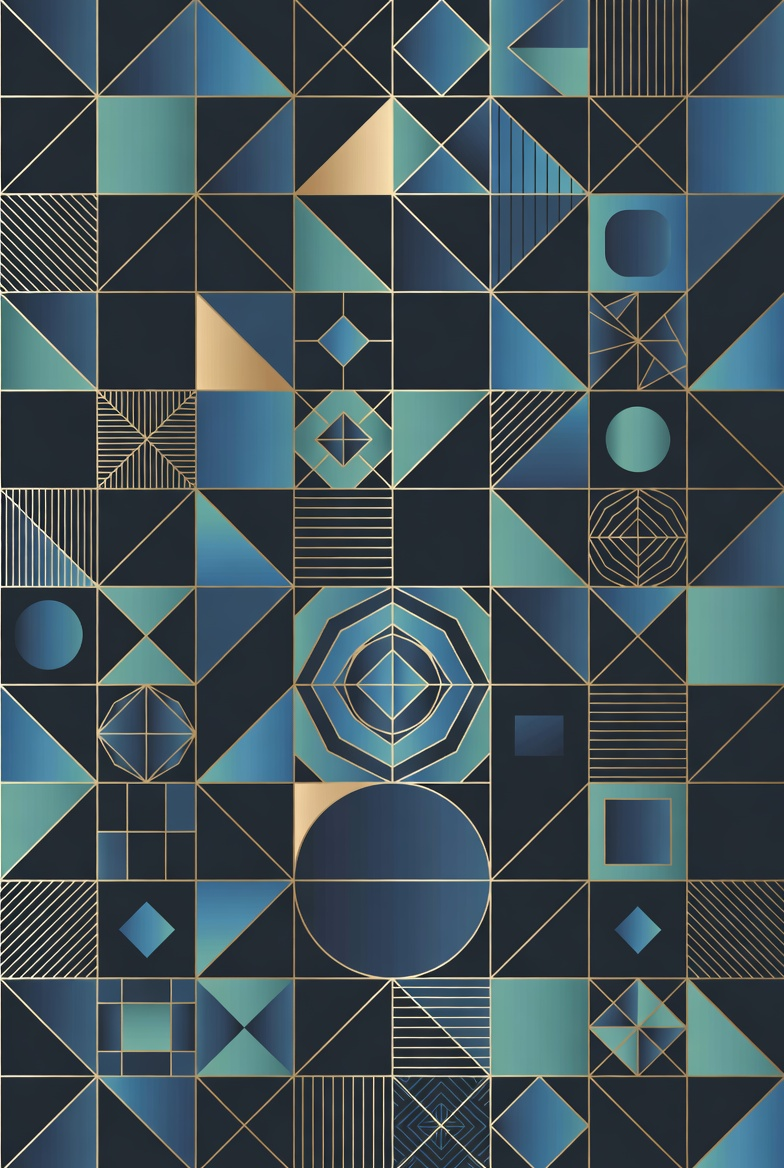
\includegraphics[width=\paperwidth,height=\paperheight]{cover.jpg}
  };

  % タイトル帯（下部に半透明の黒い帯）
  \fill[black,opacity=0.55]
    (current page.south west) rectangle ([yshift=85mm]current page.south east);

  % タイトル文字（左下基準で大きく）
  \node[anchor=south west, text=white] at ([xshift=18mm,yshift=18mm]current page.south west) {%
    \begin{minipage}{0.86\paperwidth}
      {\fontsize{32}{38}\selectfont\bfseries \BookTitle \par}
      \vspace{3mm}
      {\fontsize{16}{20}\selectfont \BookSubtitle \par}
      \vspace{6mm}
      {\fontsize{12}{14}\selectfont \BookAuthor \quad / \quad \BookCircle \par}
      {\fontsize{10}{12}\selectfont \BookVersion \quad / \quad \BookDate \par}
    \end{minipage}
  };
\end{tikzpicture}

\clearpage

% 余白設定を元に戻す
\restoregeometry

% 本文開始：ここからページ番号を 1 に
\setcounter{page}{1}
